\documentclass[
  jou,
  floatsintext,
  longtable,
  a4paper,
  nolmodern,
  notxfonts,
  notimes,
  colorlinks=true,linkcolor=blue,citecolor=blue,urlcolor=blue]{apa7}

\usepackage{amsmath}
\usepackage{amssymb}



\usepackage[bidi=default]{babel}
\babelprovide[main,import]{spanish}
\StartBabelCommands{spanish}{captions} [unicode, fontenc=TU EU1 EU2, charset=utf8] \SetString{\keywordname}{Palabras
Claves}
\EndBabelCommands


% get rid of language-specific shorthands (see #6817):
\let\LanguageShortHands\languageshorthands
\def\languageshorthands#1{}

\RequirePackage{longtable}
\RequirePackage{threeparttablex}

\makeatletter
\renewcommand{\paragraph}{\@startsection{paragraph}{4}{\parindent}%
	{0\baselineskip \@plus 0.2ex \@minus 0.2ex}%
	{-.5em}%
	{\normalfont\normalsize\bfseries\typesectitle}}

\renewcommand{\subparagraph}[1]{\@startsection{subparagraph}{5}{0.5em}%
	{0\baselineskip \@plus 0.2ex \@minus 0.2ex}%
	{-\z@\relax}%
	{\normalfont\normalsize\bfseries\itshape\hspace{\parindent}{#1}\textit{\addperi}}{\relax}}
\makeatother




\usepackage{longtable, booktabs, multirow, multicol, colortbl, hhline, caption, array, float, xpatch}
\setcounter{topnumber}{2}
\setcounter{bottomnumber}{2}
\setcounter{totalnumber}{4}
\renewcommand{\topfraction}{0.85}
\renewcommand{\bottomfraction}{0.85}
\renewcommand{\textfraction}{0.15}
\renewcommand{\floatpagefraction}{0.7}

\usepackage{tcolorbox}
\tcbuselibrary{listings,theorems, breakable, skins}
\usepackage{fontawesome5}

\definecolor{quarto-callout-color}{HTML}{909090}
\definecolor{quarto-callout-note-color}{HTML}{0758E5}
\definecolor{quarto-callout-important-color}{HTML}{CC1914}
\definecolor{quarto-callout-warning-color}{HTML}{EB9113}
\definecolor{quarto-callout-tip-color}{HTML}{00A047}
\definecolor{quarto-callout-caution-color}{HTML}{FC5300}
\definecolor{quarto-callout-color-frame}{HTML}{ACACAC}
\definecolor{quarto-callout-note-color-frame}{HTML}{4582EC}
\definecolor{quarto-callout-important-color-frame}{HTML}{D9534F}
\definecolor{quarto-callout-warning-color-frame}{HTML}{F0AD4E}
\definecolor{quarto-callout-tip-color-frame}{HTML}{02B875}
\definecolor{quarto-callout-caution-color-frame}{HTML}{FD7E14}

%\newlength\Oldarrayrulewidth
%\newlength\Oldtabcolsep


\usepackage{hyperref}




\providecommand{\tightlist}{%
  \setlength{\itemsep}{0pt}\setlength{\parskip}{0pt}}
\usepackage{longtable,booktabs,array}
\usepackage{calc} % for calculating minipage widths
% Correct order of tables after \paragraph or \subparagraph
\usepackage{etoolbox}
\makeatletter
\patchcmd\longtable{\par}{\if@noskipsec\mbox{}\fi\par}{}{}
\makeatother
% Allow footnotes in longtable head/foot
\IfFileExists{footnotehyper.sty}{\usepackage{footnotehyper}}{\usepackage{footnote}}
\makesavenoteenv{longtable}

\usepackage{graphicx}
\makeatletter
\newsavebox\pandoc@box
\newcommand*\pandocbounded[1]{% scales image to fit in text height/width
  \sbox\pandoc@box{#1}%
  \Gscale@div\@tempa{\textheight}{\dimexpr\ht\pandoc@box+\dp\pandoc@box\relax}%
  \Gscale@div\@tempb{\linewidth}{\wd\pandoc@box}%
  \ifdim\@tempb\p@<\@tempa\p@\let\@tempa\@tempb\fi% select the smaller of both
  \ifdim\@tempa\p@<\p@\scalebox{\@tempa}{\usebox\pandoc@box}%
  \else\usebox{\pandoc@box}%
  \fi%
}
% Set default figure placement to htbp
\def\fps@figure{htbp}
\makeatother







\usepackage{newtx}

\defaultfontfeatures{Scale=MatchLowercase}
\defaultfontfeatures[\rmfamily]{Ligatures=TeX,Scale=1}





\title{Cadena de suministros}


\shorttitle{Gestión de la cadena de suministros}


\usepackage{etoolbox}



\ccoppy{\textcopyright~2025}



\author{Edison Achalma}



\affiliation{
{Escuela Profesional de Economía, Universidad Nacional de San Cristóbal
de Huamanga}}




\leftheader{Achalma}

\date{2022-01-23}


\abstract{The supply chain management (SCM) is a critical framework for
coordinating business processes across multiple entities, including
suppliers, manufacturers, distributors, and retailers. This article
explores the main stages of the supply chain---sourcing, manufacturing,
distribution, and consumption---and their integration to deliver
products efficiently to consumers. It examines how these stages interact
to minimize costs while meeting customer demands. Additionally, the
study categorizes supply chains into three types: industrial,
commercial, and service-based enterprises, highlighting their distinct
operational characteristics. Using the tuna supply chain as an example,
the article illustrates global coordination among fishing fleets,
intermediaries, manufacturers, and retailers, emphasizing the role of
transportation workers. Drawing from established literature, the
analysis underscores the importance of intra- and inter-organizational
synergy in modern supply chain management. The findings aim to provide a
comprehensive understanding of supply chain dynamics for students and
practitioners in business and logistics. }

\keywords{supply chain management, business
processes, logistics, enterprise types, global coordination}

\authornote{\par{\addORCIDlink{Edison Achalma}{0000-0001-6996-3364}} 
\par{ }
\par{   El autor no tiene conflictos de interés que revelar.    Los
roles de autor se clasificaron utilizando la taxonomía de roles de
colaborador (CRediT; https://credit.niso.org/) de la siguiente
manera:  Edison Achalma:   conceptualización, redacción}
\par{La correspondencia relativa a este artículo debe dirigirse a Edison
Achalma, Email: \href{mailto:elmer.achalma.09@unsch.edu.pe}{elmer.achalma.09@unsch.edu.pe}}
}

\usepackage{pbalance} 
\usepackage{float}
\makeatletter
\let\oldtpt\ThreePartTable
\let\endoldtpt\endThreePartTable
\def\ThreePartTable{\@ifnextchar[\ThreePartTable@i \ThreePartTable@ii}
\def\ThreePartTable@i[#1]{\begin{figure}[!htbp]
\onecolumn
\begin{minipage}{0.5\textwidth}
\oldtpt[#1]
}
\def\ThreePartTable@ii{\begin{figure}[!htbp]
\onecolumn
\begin{minipage}{0.5\textwidth}
\oldtpt
}
\def\endThreePartTable{
\endoldtpt
\end{minipage}
\twocolumn
\end{figure}}
\makeatother


\makeatletter
\let\endoldlt\endlongtable		
\def\endlongtable{
\hline
\endoldlt}
\makeatother

\newenvironment{twocolumntable}% environment name
{% begin code
\begin{table*}[!htbp]%
\onecolumn%
}%
{%
\twocolumn%
\end{table*}%
}% end code

\urlstyle{same}



\makeatletter
\@ifpackageloaded{caption}{}{\usepackage{caption}}
\AtBeginDocument{%
\ifdefined\contentsname
  \renewcommand*\contentsname{Tabla de contenidos}
\else
  \newcommand\contentsname{Tabla de contenidos}
\fi
\ifdefined\listfigurename
  \renewcommand*\listfigurename{Listado de Figuras}
\else
  \newcommand\listfigurename{Listado de Figuras}
\fi
\ifdefined\listtablename
  \renewcommand*\listtablename{Listado de Tablas}
\else
  \newcommand\listtablename{Listado de Tablas}
\fi
\ifdefined\figurename
  \renewcommand*\figurename{Figura}
\else
  \newcommand\figurename{Figura}
\fi
\ifdefined\tablename
  \renewcommand*\tablename{Tabla}
\else
  \newcommand\tablename{Tabla}
\fi
}
\@ifpackageloaded{float}{}{\usepackage{float}}
\floatstyle{ruled}
\@ifundefined{c@chapter}{\newfloat{codelisting}{h}{lop}}{\newfloat{codelisting}{h}{lop}[chapter]}
\floatname{codelisting}{Listado}
\newcommand*\listoflistings{\listof{codelisting}{Listado de Listados}}
\makeatother
\makeatletter
\makeatother
\makeatletter
\@ifpackageloaded{caption}{}{\usepackage{caption}}
\@ifpackageloaded{subcaption}{}{\usepackage{subcaption}}
\makeatother
\makeatletter
\@ifpackageloaded{fontawesome5}{}{\usepackage{fontawesome5}}
\makeatother

% From https://tex.stackexchange.com/a/645996/211326
%%% apa7 doesn't want to add appendix section titles in the toc
%%% let's make it do it
\makeatletter
\xpatchcmd{\appendix}
  {\par}
  {\addcontentsline{toc}{section}{\@currentlabelname}\par}
  {}{}
\makeatother

%% Disable longtable counter
%% https://tex.stackexchange.com/a/248395/211326

\usepackage{etoolbox}

\makeatletter
\patchcmd{\LT@caption}
  {\bgroup}
  {\bgroup\global\LTpatch@captiontrue}
  {}{}
\patchcmd{\longtable}
  {\par}
  {\par\global\LTpatch@captionfalse}
  {}{}
\apptocmd{\endlongtable}
  {\ifLTpatch@caption\else\addtocounter{table}{-1}\fi}
  {}{}
\newif\ifLTpatch@caption
\makeatother

\begin{document}

\maketitle

\hypertarget{toc}{}
\tableofcontents
\newpage
\section[Introduction]{Cadena de suministros}

\setcounter{secnumdepth}{-\maxdimen} % remove section numbering

\setlength\LTleft{0pt}


\section{Cadena de suministros}\label{cadena-de-suministros}

\subsection{Conceptos básicos}\label{conceptos-buxe1sicos}

Según Lambert (1998), la administración de la cadena de suministro (SCM,
por sus siglas en inglés), se introdujo originalmente por consultores a
principio de los ochentas y subsecuentemente ha ganado mucha atención.

La cadena de suministro no es una cadena de negocios de persona a
persona, ni de relaciones entre una empresa y otra, sino que es una red
de unidades de negocio con relaciones múltiples. Ofreciendo la
oportunidad de capturar la sinergia de la integración administrativa
intra e interempresarial. En ese sentido, consiste en procesos de
excelencia y representa una nueva manera de manejar las transacciones
comerciales y relaciones con otras unidades de negocio Chase, et.al.
(2009).

Conjunto de empresas eficientemente integradas por los proveedores, los
fabricantes, distribuidores y vendedores mayoristas o detallistas
coordinados que busca ubicar uno o más productos en las cantidades
correctas, en los lugares correctos y en el tiempo preciso, buscando el
menor costo de las actividades de valor de los integrantes de la cadena
y satisfacer los requerimientos de los consumidores. Lambert y Pohlen,
(2001).

\subsection{Etapas de la Cadena de
Suministro}\label{etapas-de-la-cadena-de-suministro}

\begin{figure}[!htbp]

{\caption{{Etapas de la cadena de
Abastecimiento}{\label{fig-myimportedimage}}}}

\pandocbounded{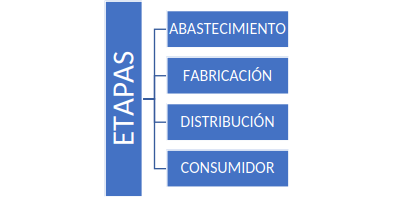
\includegraphics[keepaspectratio]{index_files/figure-html/image-20250330132806207.png}}

{\noindent \emph{Note.} Adaptación de acuerdo a Chopra y Meindel (2008)}

\end{figure}

\subsubsection{Abastecimiento o
suministro:}\label{abastecimiento-o-suministro}

Se encarga del cómo y dónde obtener las materias primas, dónde
almacenarlas, cómo movilizarlas y qué criterios emplear en su selección.

La etapa de abastecimiento se concentra en cómo, donde y cuando se
consiguen y suministran las materias primas para fabricación de los
productos terminados. Es la etapa relacionada con la función de compra,
adquisición o abastecimiento de materias primas, insumos y soluciones
complejas para el desarrollo de las actividades de fabricación o
producción Bowersox et al., (2007).

\subsubsection{Fabricación:}\label{fabricaciuxf3n}

Es el momento en sí de hacer físico el producto. Producirlo y hacerlo
real.

En esta etapa se convierten las materias primas en productos terminados.
Más allá del proceso propio de producción que una compañía manufacturera
o de servicios pueda establecer, la cadena de abastecimiento se enfoca
en definir los procesos que existe entre esta etapa de la cadena y la
etapa de abastecimiento y posteriormente la de distribuidores. De esta
forma las empresas, deben establecer canales que les ETAPAS
ABASTECIMIENTO FABRICACIÓN DISTRIBUCIÓN CONSUMIDOR Cadenas de Suministro
15 permitan controlar los frentes importantes que una cadena de
abastecimiento requiera, las cuales se pueden consolidar en las etapas
Cala, (2005).

\subsubsection{Distribución:}\label{distribuciuxf3n}

Con el producto ya acabado es el momento de almacenarlo a la espera de
que pase por el control de calidad.

Se encarga de que dichos productos terminados lleguen al consumidor
atreves de una red de distribuidores, almacenes y comercios minoristas.
Una vez finalizado el proceso de producción el producto final debe ser
transportado hasta su destino final, de acuerdo con el acuerdo realizado
entre el productor y el cliente, quienes determinan el lugar de entrega
y el medio de transporte para su llegada Díaz et al., (2008).

\subsubsection{Consumidor:}\label{consumidor}

Con la mercadería ya acabada y controlado ahora queda distribuirlo a los
diferentes puntos de venta.

Es una persona u organización que demanda bienes o servicios
proporcionados por el productor o el proveedor de bienes o servicios. Es
decir, es cualquiera que se ve afectado por el servicio, el producto o
el proceso Juran J. (2007).

\subsection{Tipos de cadenas de
suministros}\label{tipos-de-cadenas-de-suministros}

\subsubsection{Empresas industriales:}\label{empresas-industriales}

Tienen una \textbf{cadena de suministro} con mucha logística, que
dependerán del tamaño de la empresa, de las líneas de producción con que
cuentan y mercado al que van dirigidos sus productos. Generalmente
incluye funciones como, desarrollo de nuevos productos, la
mercadotecnia, importación, fabricación, la distribución, las finanzas y
el servicio al cliente.

\subsubsection{Empresas
comercializadoras:}\label{empresas-comercializadoras}

En este caso son menos elaboradas, no maneja la parte productiva, maneja
mayormente la obtención y venta de productos. Abarca funciones
destinadas a la recepción de una solicitud del cliente y el cumplimiento
de dicha solicitud.

\subsubsection{Empresas de servicios:}\label{empresas-de-servicios}

Estas cuentan con cadenas muy cortas. Es más, una cadena jerárquica y
depende del recurso humano.

\subsection{Ejemplo de las cadenas de suministro del
atún}\label{ejemplo-de-las-cadenas-de-suministro-del-atuxfan}

La gran mayoría del atún en lata se produce para los mercados de Europa
y Estados Unidos. Por ende, el consumo de atún en Estados Unidos y
Europa depende de las cadenas de suministro mundiales en las que
participan:

\begin{itemize}
\tightlist
\item
  Las flotas encargadas de la pesca.\\
\item
  Los comerciantes que actúan como intermediarios entre las flotas
  pesqueras y los fabricantes.\\
\item
  Los fabricantes que procesan y envasan el pescado.\\
\item
  Los minoristas que venden el pescado al consumidor final
\end{itemize}

\begin{figure}[H]

\caption{Cadenas de suministro del atún}

{\centering \pandocbounded{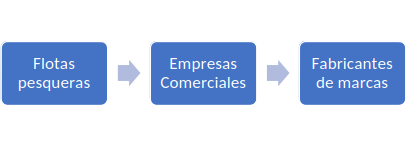
\includegraphics[keepaspectratio]{index_files/figure-html/image-20250330133145909.png}}

}

\end{figure}%

Los trabajadores del transporte desempeñan un papel de suma importancia
en estas cadenas de suministro. Estas etapas están conectadas entre sí
por trabajadores/as del transporte que trasladan el atún por carretera,
ferrocarril, mar y aire entre empresas y ubicaciones.

\subsection{Bibliografías}\label{bibliografuxedas}

Bowersox , D.J.(2007): \emph{Administración y logística en la cadena de
suministros, adquisición y fabricación Bixby.} Mc Graw Hill, México.

Cala, A.(2005): \emph{Revista Electrónica CIVILIZAR} Universidad Sergio
Arboleda, Sección Finanzas.

Chase, Richard, Jacobs, Robert, Aquilano, Nicholas (2009).
\emph{Administración de operaciones: Producción y cadena de
suministros.} Decima edición. McGraw-Hill.

Díaz Hector; Garcia Rafael; Porcell Nestor (2008): \emph{Las Pymes:
Costos en la cadena de abastecimientos. Revista- escuela de
administración de negocios,} Núm. 63, Mayo-Agosto 2008, pp.~5-21
Universidad EAN Colombia Redalyc.

Juran Joseph, Gryna Frank, Chua Richard, Defeo Josep (2007).
\emph{Análisis y planeación de la calidad, quinta edición.}

Lambert, D.M., Cooper, M.C., Pagh, J.D., (1998). \emph{Supply
opportunities.En: The international journal of logistics management},
vol.2, p1.

Lambert, Douglas M. y Pohlen, Terrance (2001). \emph{Supply Chain
Metric. The International Journal of Logistics Management,} Volume 12,
Number 1.

\section{Publicaciones Similares}\label{publicaciones-similares}

Si te interesó este artículo, te recomendamos que explores otros blogs y
recursos relacionados que pueden ampliar tus conocimientos. Aquí te dejo
algunas sugerencias:

\begin{enumerate}
\def\labelenumi{\arabic{enumi}.}
\tightlist
\item
  \href{https://achalmaedison.netlify.app/blog/posts/2015-05-14-el-aborto/index.pdf}{\faIcon{file-pdf}}
  \href{https://achalmaedison.netlify.app/blog/posts/2015-05-14-el-aborto}{El
  Aborto}
\item
  \href{https://achalmaedison.netlify.app/blog/posts/2017-04-23-sitios-web-asombrosos/index.pdf}{\faIcon{file-pdf}}
  \href{https://achalmaedison.netlify.app/blog/posts/2017-04-23-sitios-web-asombrosos}{Sitios
  Web Asombrosos}
\item
  \href{https://achalmaedison.netlify.app/blog/posts/2017-05-23-el-mercantilismo/index.pdf}{\faIcon{file-pdf}}
  \href{https://achalmaedison.netlify.app/blog/posts/2017-05-23-el-mercantilismo}{El
  Mercantilismo}
\item
  \href{https://achalmaedison.netlify.app/blog/posts/2020-05-23-comandos-de-google-assistant/index.pdf}{\faIcon{file-pdf}}
  \href{https://achalmaedison.netlify.app/blog/posts/2020-05-23-comandos-de-google-assistant}{Comandos
  De Google Assistant}
\item
  \href{https://achalmaedison.netlify.app/blog/posts/2020-09-15-plan-de-negocio-exportacion-de-trucha-arcoires/index.pdf}{\faIcon{file-pdf}}
  \href{https://achalmaedison.netlify.app/blog/posts/2020-09-15-plan-de-negocio-exportacion-de-trucha-arcoires}{Plan
  De Negocio Exportacion De Trucha Arcoires}
\item
  \href{https://achalmaedison.netlify.app/blog/posts/2021-07-13-plan-de-negocio-exportacion-de-tuna/index.pdf}{\faIcon{file-pdf}}
  \href{https://achalmaedison.netlify.app/blog/posts/2021-07-13-plan-de-negocio-exportacion-de-tuna}{Plan
  De Negocio Exportacion De Tuna}
\item
  \href{https://achalmaedison.netlify.app/blog/posts/2021-07-14-comandos-de-blogdown/index.pdf}{\faIcon{file-pdf}}
  \href{https://achalmaedison.netlify.app/blog/posts/2021-07-14-comandos-de-blogdown}{Comandos
  De Blogdown}
\item
  \href{https://achalmaedison.netlify.app/blog/posts/2021-10-01-gestion-publica-y-administracion-publica/index.pdf}{\faIcon{file-pdf}}
  \href{https://achalmaedison.netlify.app/blog/posts/2021-10-01-gestion-publica-y-administracion-publica}{Gestion
  Publica Y Administracion Publica}
\item
  \href{https://achalmaedison.netlify.app/blog/posts/2021-10-01-reformas-y-modernizacion-de-la-gestion-publica/index.pdf}{\faIcon{file-pdf}}
  \href{https://achalmaedison.netlify.app/blog/posts/2021-10-01-reformas-y-modernizacion-de-la-gestion-publica}{Reformas
  Y Modernizacion De La Gestion Publica}
\item
  \href{https://achalmaedison.netlify.app/blog/posts/2022-01-23-cadena\%20de\%20suministros/index.pdf}{\faIcon{file-pdf}}
  \href{https://achalmaedison.netlify.app/blog/posts/2022-01-23-cadena\%20de\%20suministros}{Cadena
  De Suministros}
\item
  \href{https://achalmaedison.netlify.app/blog/posts/2022-04-22-economia-agraria/index.pdf}{\faIcon{file-pdf}}
  \href{https://achalmaedison.netlify.app/blog/posts/2022-04-22-economia-agraria}{Economia
  Agraria}
\item
  \href{https://achalmaedison.netlify.app/blog/posts/2022-06-02-impacto-del-cambio-climatico/index.pdf}{\faIcon{file-pdf}}
  \href{https://achalmaedison.netlify.app/blog/posts/2022-06-02-impacto-del-cambio-climatico}{Impacto
  Del Cambio Climatico}
\item
  \href{https://achalmaedison.netlify.app/blog/posts/2023-05-11-cualidades-de-los-servidores-publicos/index.pdf}{\faIcon{file-pdf}}
  \href{https://achalmaedison.netlify.app/blog/posts/2023-05-11-cualidades-de-los-servidores-publicos}{Cualidades
  De Los Servidores Publicos}
\item
  \href{https://achalmaedison.netlify.app/blog/posts/2023-05-12-la-economia-peruana-entre-1970-1990/index.pdf}{\faIcon{file-pdf}}
  \href{https://achalmaedison.netlify.app/blog/posts/2023-05-12-la-economia-peruana-entre-1970-1990}{La
  Economia Peruana Entre 1970 1990}
\item
  \href{https://achalmaedison.netlify.app/blog/posts/2023-05-16-economia-regional/index.pdf}{\faIcon{file-pdf}}
  \href{https://achalmaedison.netlify.app/blog/posts/2023-05-16-economia-regional}{Economia
  Regional}
\end{enumerate}

Esperamos que encuentres estas publicaciones igualmente interesantes y
útiles. ¡Disfruta de la lectura!






\end{document}
